\model{Linked Lists}

Linked structures ``chain'' elements using references.
Each element of the list is called a \emph{node}.

\vspace{1ex}
\begin{minipage}{0.40\linewidth}
\begin{javalst}
    public class Node
    {
        private int value;
        private Node next;
        ...
    }
\end{javalst}
\end{minipage}
\hfill
\begin{minipage}{0.58\linewidth}
\begin{javalst}
    Node node3 = new Node(14, null);
    Node node2 = new Node(6, node3);
    Node numbers = new Node(22, node2);
\end{javalst}
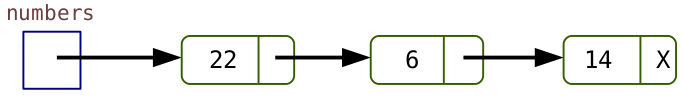
\includegraphics[scale=0.35]{figs/list1.png}
\end{minipage}
\vspace{1em}

This organization allows fast insertions/deletions near the beginning. For example, to add 8:

\vspace{1ex}
\begin{minipage}{0.48\linewidth}
\begin{javalst}
    Node temp = new Node(8, numbers);



    numbers = temp;
\end{javalst}
\end{minipage}
\hfill
\begin{minipage}{0.50\linewidth}
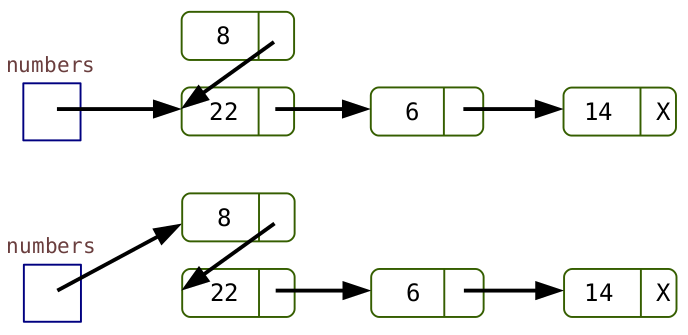
\includegraphics[scale=0.35]{figs/list2.png}
\end{minipage}
\vspace{1em}

Instead of working with nodes directly, we can design a wrapper class to handle list logic:

\vspace{1ex}
\begin{minipage}{0.40\linewidth}
\begin{javalst}
    public class MyList
    {
        private int size;
        private Node head;
        ...
    }
\end{javalst}
\end{minipage}
\hfill
\begin{minipage}{0.58\linewidth}
\begin{javalst}
    MyList numbers = new MyList();
    numbers.addAtStart(14);
    numbers.addAtStart(6);
    numbers.addAtStart(22);
\end{javalst}
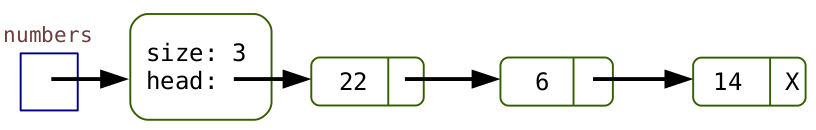
\includegraphics[scale=0.35]{figs/list3.png}
\end{minipage}
\vspace{1ex}


\quest{15 min}


\Q How many assignment operations are required to add 14 {\it at the front} of an empty list? Note that creating a \java{Node} takes two assignments (one for \java{value} and one for \java{next}).

\begin{answer}
3 operations: 1 to assign the \java{value}, 1 to assign null to \java{next}, and 1 to assign the reference of the new Node to the head variable (node3 in this case).
\end{answer}


\Q How many operations are required to add 22 at the front, after 14 and 6 have been added?

\begin{answer}
Still just 3, in fact the same as the first insert. Note that no shifting is required.
\end{answer}


\Q Using this model, how many operations are required to add another element {\it at the end} of the current list?

\begin{answer}[3em]
5 operations: 3 to find where the new element goes (by following references to the end of the list), one to create the new node, and one to change the reference of the previous last element.
\end{answer}


\Q How much memory is needed to store each element in the \java{LinkedList}?
How does that amount compare with using an \java{ArrayList}?

\begin{answer}
Linked lists need to store two references per node (one for \java{value} and one for \java{next}).
In contrast, array lists only need to store the \java{value} references.
At a conceptual level, array lists take up about half as much space as linked lists (not counting empty cells and object overhead).
\end{answer}


\Q \label{LinksAreBad}
Discuss why \java{LinkedList} is a poor choice of \java{List} in the program below.

\vspace{1ex}
\begin{javabox}
import java.util.LinkedList;
import java.util.List;

public class LinksAreBad
{
    public static void main(String[] args)
    {
        LinkedList<String> linkedList = new LinkedList<>();

        System.out.println("LinkedList: ");
        addAndGet(linkedList);
        System.out.println("Done!");
    }

    public static void addAndGet(List<String> list)
    {
        for (int i = 0; i < 1000000; i++)
        {
            list.add("A");  // add at the end
        }

        for (int i = 0; i < 1000000; i++)
        {
            list.get(list.size() / 2);  // get the middle element
        }
    }
}
\end{javabox}
\vspace{-1ex}

\begin{answer}[3em]
Each insertion in the middle of the list takes $n/2$ operations (where $n$ is the current size of the collection) in order to find the \java{next} references to assign.
\end{answer}
